\scanpage{44}
\mspage{\handwritten{12}}
\uline{Définition 11.3.}- Etant donné un $S$-groupe $G$ plat, quasi-compact et quasi-séparé sur $S$, tel que $\handwritten{\unsure{\mathcal{A}|a}}(G)$ soit plat sur $\handwritten{\mathcal{O}}_S$, nous noterons $G_{\mathrm{af}}$ , et nous appellerons \uline{enveloppe affine} de $G$ le $S$-groupe $G_{\mathrm{af}}=\operatorname{Spec}\handwritten{\mathcal{A}}(G)$.
\margin{\deleted{\handwritten{\unsure{vu}}}}

\uline{11.4.}- Etant donnés deux $\handwritten{\mathcal{O}}_S$-Modules $\handwritten{\mathcal{E}}$ et $\handwritten{\mathcal{F}}$ quasi-cohérents, notons $\handwritten{\mathcal{H}om}_S(\handwritten{\mathbb{V}}(\handwritten{\mathcal{F}}),\handwritten{\mathbb{V}}(\handwritten{\mathcal{E}}))$ le $S$-foncteur des morphismes de $S$-foncteurs de $\handwritten{\mathbb{V}}(\handwritten{\mathcal{F}})$ dans $\handwritten{\mathbb{V}}(\handwritten{\mathcal{E}})$, et $\handwritten{\mathcal{H}om}_{\handwritten{\mathcal{O}}_S}(\handwritten{\mathbb{V}}(\handwritten{\mathcal{F}}),\handwritten{\mathbb{V}}(\handwritten{\mathcal{E}}))$ le sous-$S$-foncteur de $\handwritten{\mathcal{H}om}_S(\handwritten{\mathbb{V}}(\handwritten{\mathcal{F}}),\handwritten{\mathbb{V}}(\handwritten{\mathcal{E}}))$ formé des $\handwritten{\mathcal{O}}_S$- homomorphismes de $\handwritten{\mathcal{O}}_S$-foncteurs en modules (cf. \deleted{Exp.} I). Alors $\handwritten{\mathcal{H}om}_{\handwritten{\mathcal{O}}_S}(\handwritten{\mathbb{V}}(\handwritten{\mathcal{F}}),\handwritten{\mathbb{V}}(\handwritten{\mathcal{E}}))(T)$ est en correspondance bi\deleted{n}\inserted{\handwritten{un}}ivoque canonique avec $\deleted{\unsure{\operatorname{Hom}}}\operatorname{Hom}_{\handwritten{\mathcal{O}}_{S\deleted{\unsure{T}}}\text{-}\mathrm{Mod.}}(\handwritten{\mathcal{E}\otimes}_{\handwritten{\mathcal{O}}_S}\handwritten{\mathcal{O}}_T,\deleted{\unsure{(}}\handwritten{\mathcal{F}\otimes}_{\handwritten{\mathcal{O}}_S}\handwritten{\mathcal{O}}_T\deleted{\unsure{)}}$,
\inserted{\handwritten{$\text{i.e.}\quad \mathcal{H}om_{\underline{O}_S}(\mathbb{V}(\mathcal{F}),\mathbb{V}(\mathcal{E}))\simeq\mathcal{H}om_{\underline{O}_S}(\mathbb{W}(\mathcal{E}),\mathbb{W}(\mathcal{F})).$}}
\margin{\handwritten{\unsure{vu}}}

Soit $X$ un $S$-préschéma. Alors l'ensemble des morphismes de $S$-foncteurs de $X$ dans $\handwritten{\mathcal{H}om}_S(\deleted{\handwritten{\unsure{\mathbb{V}|W}}}\handwritten{\mathbb{V}}(\handwritten{\mathcal{F}}),\handwritten{\mathbb{V}}(\handwritten{\mathcal{E}}))$ est en correspondance bi\inserted{\handwritten{un}}nivoque avec $\operatorname{Hom}_S(X\handwritten{\times}_S\handwritten{\mathbb{V}}(\handwritten{\mathcal{F}}),\handwritten{\mathbb{V}}(\handwritten{\mathcal{E}}))$, donc l'ensemble des morphismes de $S$-foncteurs de $X$ dans $\handwritten{\mathcal{H}om}_{\handwritten{\mathcal{O}}_S}(\handwritten{\mathbb{V}}(\handwritten{\mathcal{F}}),\handwritten{\mathbb{V}}(\handwritten{\mathcal{E}}))$ est en correspondance biunivoque avec un sous-ensemble de $\operatorname{Hom}_S(X\handwritten{\times}_S\handwritten{\mathbb{V}}(\handwritten{\mathcal{F}}),\handwritten{\mathbb{V}}(\handwritten{\mathcal{E}}))=\operatorname{Hom}_{\handwritten{\mathcal{O}}_S\text{-}\mathrm{Mod;}}(\handwritten{\mathcal{E}},\handwritten{\mathcal{A}}(X\handwritten{\times}_S\handwritten{\mathbb{V}}(\handwritten{\mathcal{F}})))$ (EGA II 1.7.13).

\uline{Proposition 11.5.- Soient $X$ un $S$-p\handwritten{\makebox[0pt][l]{\begin{tikzpicture}[x=.2cm,y=.2cm,baseline=-.3ex]\draw (0,-.2) .. controls (.35,0) and (.55,.4) .. (.8,.4);\end{tikzpicture}}}réschéma quasi-compact quasi-séparé sur $S$, $f:X\handwritten{\to}S$ le morphisme structural, $\handwritten{\mathcal{E}}$ et $\handwritten{\mathcal{F}}$ deux $\handwritten{\mathcal{O}}_S$-Modules quasi-cohérents. On suppose vérifiée\deleted{s} l'une des deux conditions suivantes :}

\uline{a) $f$ est affine}

\uline{b) $\handwritten{\mathcal{F}}$ est plat sur $\handwritten{\mathcal{O}}_S$.}

\uline{Alors :}

\margin{\handwritten{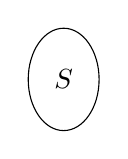
\begin{tikzpicture}\draw (0,0) ellipse (.45 and .65);\node at (0,0) {$S$};\end{tikzpicture}}}
\uline{i) l'homomorphisme canonique $\handwritten{\varphi:\mathcal{A}}(X)\handwritten{\otimes}_{\handwritten{\mathcal{O}}_S}\handwritten{\mathbb{S}}(\handwritten{\mathcal{F}})\handwritten{\longrightarrow\mathcal{A}}(X\handwritten{\times}_S\handwritten{\mathbb{V}}(\handwritten{\mathcal{F}}))$ est un isomorphisme (où $\handwritten{\mathbb{S}}(\handwritten{\mathcal{F}})$ désigne l'Algèbre symétrique de $\handwritten{\mathcal{F}}$).}

\uline{ii) l'ensemble des morphismes de $S$-foncteurs de $X$ dans $\handwritten{\mathcal{H}om}_{\handwritten{\mathcal{O}}_S}(\handwritten{\mathbb{V}}(\handwritten{\mathcal{F}}),\handwritten{\mathbb{V}}(\handwritten{\mathcal{E}}))$ est en correspondance biunivoque avec $\operatorname{Hom}_{\handwritten{\mathcal{O}}_S\text{-}\mathrm{Mod.}}(\handwritten{\mathcal{E}}\ ,\ \handwritten{\mathcal{A}}(X)\handwritten{\otimes\mathcal{F}})$.}

Pour montrer i), d'après (11.1, a) et b)), il suffit de montrer que si $\handwritten{\mathcal{F}}$ est plat sur $\handwritten{\mathcal{O}}_{\unsure{\mathbb{S}|S}}$, \deleted{il en est de même de $\handwritten{\mathbb{S}}(\handwritten{\mathcal{F}})$} alors $\handwritten{\mathbb{V}}(\handwritten{\mathcal{F}})$ est plat sur $S$. D'après (EGA III 1.4.15.5),
% archive sheet number: 43
